\newpage
\section{Performance considerations}
\label{sec:performance}

Performance is an integral aspect of any application and as such Roslyn doesn't escape from it either. It's not just about compiling an assembly as fast as possible: that's just one of the use cases in which Roslyn is used. Think about other scenarios such as getting quick \gls{intellisense}\footnote{Intellisense: context-aware hints as you type} or fluent syntax highlighting of text as you scroll but also affects other performance aspects such as the memory impact.

In this section we will look at a handful of techniques the Roslyn team uses to optimize the platform. These are general approaches that often apply their ideas in several areas of the codebase, sometimes through a common resource. This should indicate that these are often optimizations at a high level rather than very specific single-use optimizations. 


\subsection{Concurrency}
\label{sec:concurrency}

\epigraph{A concurrent system is one where a computation can make progress without waiting for all other computations to complete -- where more than one computation can make progress at "the same time"}{\textit{Abraham Silberschatz \\ \footnotesize{Operating System Concepts 9th edition}}}

When you think of performance, concurrency is often one of the first aspects that come to mind. As such, it also takes a prominent place in Roslyn's architecture. We have already established that one of the characteristics of a \gls{syntaxtree} is its \glslink{immutable}{immutability} -- the inability to make changes to it after it is constructed. This is done with concurrency in mind: if we create a new tree for every concurrent operation, we have the guarantee that changes from operation X does not affect the tree that is being manipulated by operation Y. There are several more areas of concurrency though:

\subsubsection{Source parsing}
\label{sec:concur-source-parsing}

Every file containing source code is parsed independently of any other files. The file is parsed sequentially (from top to bottom) and multiple files can be parsed at once.\parencite{Sadov2014}

\subsubsection{Symbol binding }
\label{sec:concur-symbol-binding}

When identifiers are bound to symbols (see Chapter \ref{sec:binding-phase}) there is no real need to do this sequentially: in the end you basically just lookup the symbol in a table according to an identifier. One remark we have to add here though is the fact that a type's base members should also be bound when that type is being bound.

Consider the following example:

\lstset{style=csharp, caption={Why type hierarchy matters for binding}}
\begin{lstlisting}
class BaseType
{
	public virtual void Method() { }
	public void BaseMethod() { }	
}

class SubType : BaseType
{
	public override void Method()
	{
		base.BaseMethod();
	}
}

class AnotherType
{
	public void Method() { }
}

class StartUp 
{
	public static void Main(string[] args)
	{
		BaseType a = new SubType();
		a.Method();
		AnotherType b = new AnotherType();
		b.Method();
	}
}
\end{lstlisting}

When we bind \texttt{SubType} we have to bind \texttt{BaseType} as well because, as is indicated, there might be a semantical dependency: we have to know, for example, whether that \texttt{override} keyword is appropriate there. This is not a problem when there is no explicit base type involved: we know the base type is just \texttt{System.Object} which is likely already bound and as such there are no other types we have to investigate. For this reason we can bind unrelated symbols in no specific order. We can say there is "implicit partial ordering".\parencite{Sadov2014}

\subsubsection{Method body compilation }
\label{sec:concur-method-body-compilation}

Method bodies are bound and emitted on a type-by-type basis and in lexicographical order (based on the alphabet). This order is important: when compiling identical code multiple types it should \gls{emit} the same result every time. Sometimes compiling a method creates an additional structure such as a state machine (as is the case with async/await and iterator blocks). This idea of a 'deterministic build' is looked at more closely in section \ref{sec:deterministic-builds}. 

Important to note is that method bodies are not emitted if there were any declaration errors. If that is the case, only binding is done for those aspects that can help in diagnosing the issue.\parencite{Sadov2014}


\subsection{Small nodes}
\label{sec:small-nodes}

Another performance-oriented aspect is the so-called "memory-footprint"\footnote{Memory footprint: The amount of memory software uses when running}. When an application is executed, it uses memory to temporarily store data that makes up the program's workflow. This memory is (unfortunately) not unlimited: every device only has a certain amount available. The more memory is used, the less memory becomes available for other tasks and the sooner you run out. C\# and VB.NET are managed languages which means the allocating and freeing of memory is done for the developer. The freeing of memory is done through the "Garbage Collector" (GC), a specialized service that will free unused memory locations when it deems it to be necessary. Discussing the GC is outside of the scope of this paper but it is important to realize that the more memory we use, the more the GC will have to step in and free up some of the unused memory locations so we can re-allocate these.\parencite{Todorov2013}

Knowing that, we can take a look at the next performance aspect. As we have seen, syntax nodes are some of the most elemental constructs in our AST\footnote{AST: Abstract Syntax Tree}. Considering the sheer amount of nodes that a large applications exists of, it would pay off to keep these as small as possible. Doing so would reduce the amount of memory allocated which in turn would reduce the amount of garbage collections. A garbage collection is a relatively expensive operation since you basically put a hold on all active threads (except for the GC thread) so the GC can do its work.\parencite{Botelho2014}

For this reason the Roslyn team decided to store certain information related to syntax nodes in a place that is not associated with that specific syntax node's object.\parencite{Sadov2014} "Meta-information" like diagnostic info and annotations are the two prime examples of this. In any given code base, most syntax nodes won't have any diagnostic information attached to them nor do they have annotations. This means that providing a field on every single syntax node object to store this information would be a waste of memory: in the end, a field with a \verb|null| value will still use some memory due to its pointer. For a 32-bit process this will be a 4-bit pointer while a 64-bit process will use an 8-bit pointer\footnote{https://msdn.microsoft.com/en-us/library/system.intptr.size(v=vs.110).aspx}. Multiply this by all the relevant syntax nodes and you reach a sizable amount of wasted memory space.

What Roslyn does instead is store the diagnostics inside the syntax node's associated syntax tree and when the diagnostic information is actually requested, it will look them up inside that tree.

\noindent This becomes clear when we take a look at the execution path in the code:

\lstset{style=csharp, caption={CSharpSyntaxNode.GetDiagnostics}}
\begin{lstlisting}
public new IEnumerable<Diagnostic> GetDiagnostics()
{
	return this.SyntaxTree.GetDiagnostics(this);
}
\end{lstlisting}

\noindent which passes it on to the following chain of calls inside the syntax tree:

\lstset{style=csharp, caption={CSharpSyntaxTree.GetDiagnostics}}
\begin{lstlisting}
GetDiagnostics(node.Green, node.Position);
EnumerateDiagnostics(greenNode, position);
new SyntaxTreeDiagnosticEnumerator(this, node, position);
\end{lstlisting}

\noindent We can see a new specific enumerator is created which will traverse the syntax tree's nodes and return any diagnostics it finds. That is not the end, however. Eventually we still have to look up the diagnostic information and we know it's not stored inside the syntax node object. We follow the execution path again and now it becomes clear:

\lstset{style=csharp, caption={SyntaxTreeDiagnosticEnumerator.MoveNext}}
\begin{lstlisting}
node.GetDiagnostics(); // node is a GreenNode
\end{lstlisting}

\lstset{style=csharp, caption={GreenNode.GetDiagnostics}}
\begin{lstlisting}
if (s_diagnosticsTable.TryGetValue(this, out diags))
\end{lstlisting}

\noindent and eventually we reach a statically defined look-up table where we connect given syntax nodes with their respective diagnostic information:

\lstset{style=csharp, caption={GreenNode.s\_diagnosticsTable}}
\begin{lstlisting}
private static readonly 
	ConditionalWeakTable<GreenNode, DiagnosticInfo[]> 
		s_diagnosticsTable =
			new ConditionalWeakTable<	GreenNode, 
																DiagnosticInfo[]>();
\end{lstlisting}

This approach comes with the caveat that when there \textit{are} diagnostics or annotations, retrieving them will be more expensive compared to just accessing a field. A trade-off had to be made here between either permanent extra memory-usage or occasionally extra look-up time and apparently the latter was decided to be the best option.

\subsection{Object re-use}
\label{sec:object-reuse}

We've already highlighted the importance of memory impact in section \ref{sec:small-nodes} by making the nodes as small as possible. There is another approach we can take to this by making \textit{duplicate} nodes take absolutely no space: we simply re-use existing objects. In this section we will mimic the experiments done by Robin Sedlaczek\parencite{Sedlaczek2015} based on an explanation by Vladimir Sadov\parencite{Sadov2014}. In the end we will have shown how we reach a red-tree façade as shown in image \ref{img:performance-node-reuse-red} while having an underlying structure as shown in image \ref{img:performance-node-reuse-green}.

\begin{figure}[h]
\centering
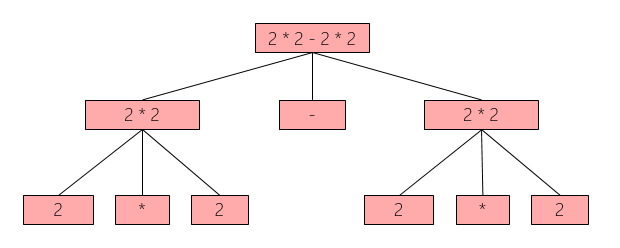
\includegraphics[scale=0.75]{performance-node-reuse-red}
\caption[Red-tree façade]{Red-tree façade \textcopyright Robin Sedlaczek}
\label{img:performance-node-reuse-red}
\end{figure}

\begin{figure}[h]
\centering
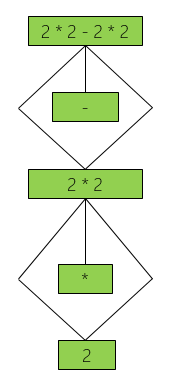
\includegraphics[scale=0.75]{performance-node-reuse-green}
\caption[Underlying green tree nodes]{Underlying green tree nodes \textcopyright Robin Sedlaczek}
\label{img:performance-node-reuse-green}
\end{figure}

\subsubsection{Re-using nodes}
\label{sec:re-use-nodes}

The first aspect we will look at is re-using our green nodes. As we established in section \ref{sec:rg-trees-solution}, green nodes have "vague" information: instead of a specific location in the syntax tree they instead contain the width of themselves. This is good because if it would have a specific location, we would (almost) never be able to re-use it: two distinct nodes in a single tree will be located at a different position. However by using the width instead we \textit{can} consider two similar nodes as identical because we merely look at their width which is the same for both.

We can demonstrate this in the following example where we look at the node that represents \texttt{2 + 2}.

\lstset{style=csharp, caption={Re-using nodes based on width vs position}}
\begin{lstlisting}
int x = 2 + 2; // Width: 5; Position: 9
int y = 2 + 2; // Width: 5; Position: 23
\end{lstlisting}

Following out of this and the fact that green nodes don't contain any other uniquely identifying information such as a parent, we can conclude that a single green node can represent multiple identical subtrees. In order to see how this is implemented we have to take a look at the \texttt{SyntaxNodeCache}\footnote{\url{https://github.com/dotnet/roslyn/blob/b908b05b41d3adc3b5e81f8cf2d0055c13e4a1f6/src/Compilers/CSharp/Portable/Syntax/InternalSyntax/SyntaxNodeCache.cs}}.

There are three main conclusions that we can take away from this implementation:

\begin{itemize}

\item Limited cache size

Only a limited amount of nodes is stored in this cache. A trade-off has to be made between execution time and memory impact and the Roslyn team has decided to use a cache size of 65536 items (\texttt{1 << 16}) as evidenced here:

\lstset{style=csharp, caption={Definition of the SyntaxNodeCache's size}}
\begin{lstlisting}
private const int CacheSizeBits = 16;
private const int CacheSize = 1 << CacheSizeBits;
private const int CacheMask = CacheSize - 1;
\end{lstlisting}

\item First In, First out

When a node is added, a hash key will be calculated. As is typical with hash implementations, this should strive to reach a uniform distribution across the data structure (an array in this case) for optimal performance. Based on this hash key and the mask, the to-be-cached node will be inserted at a certain location of the array. If an entry already exists at this location it will be overwritten, hence the FIFO (First In, First Out) principle.

\lstset{style=csharp, caption={Inserting a node using FIFO}}
\begin{lstlisting}
var idx = hash & CacheMask;
s_cache[idx] = new Entry(hash, node);
\end{lstlisting}

\item Up to 3 children

The last important aspect of this cache is the fact that every node can only have up to three children. If it has any more, the chance of a cache miss is too big\parencite{Sadov2014} so these are not allowed in the first place. This is enforced by making sure there are only overloads available for 1, 2 and 3 nodes.

\lstset{style=csharp, caption={Caching up to three children}}
\begin{lstlisting}
private static bool CanBeCached(GreenNode child1)
{
	return 	child1 == null || child1.IsCacheable;
}

private static bool CanBeCached(GreenNode child1, 
																GreenNode child2)
{
	return 	CanBeCached(child1) && 
					CanBeCached(child2);
}

private static bool CanBeCached(GreenNode child1, 
																GreenNode child2, 
																GreenNode child3)
{
	return 	CanBeCached(child1) && 
					CanBeCached(child2) && 
					CanBeCached(child3);
}
\end{lstlisting}

\end{itemize}

\subsubsection{Re-using tokens}
\label{sec:re-use-tokens}

Tokens are also cached but take a slightly different approach to doing so. When the source text is being parsed, the \texttt{QuickScanner} looks inside the \texttt{LexerCache} which maintains caches for both trivia and tokens.

\lstset{style=csharp, caption={QuickScanner.QuickScanSyntaxToken}}
\begin{lstlisting}
if (state == QuickScanState.Done)
{
	// this is a good token!
	var token = _cache.LookupToken(
	    TextWindow.CharacterWindow,
	    TextWindow.LexemeRelativeStart,
	    i - TextWindow.LexemeRelativeStart,
	    hashCode,
	    _createQuickTokenFunction);
	return token;
}
\end{lstlisting}

Inside the \texttt{LexerCache} the caches for trivia and tokens are stored by way of a \texttt{TextKeyedCache} implementation. A \texttt{TextKeyedCache} maintains two levels of caching: a local one and a shared one, each with their own characteristics.

\noindent L1 Cache:

\begin{itemize}
\item Small cache size ($2^{11}$ items)
\item Fast
\item Thread-unsafe
\item Local to the parsing session
\end{itemize}

\noindent L2 Cache:

\begin{itemize}
\item Larger cache size ($2^{16}$ items)
\item Slower
\item Thread-safe
\item Shared between all parsing sessions
\end{itemize}

\noindent When an item is searched for in the cache, the \texttt{TextKeyedCache} will first attempt to find it in the local cache (\texttt{\_localTable}) and if it wasn't found there, look in the shared cache (\texttt{s\_sharedTable}).

\lstset{style=csharp, caption={TextKeyedCache.FindItem}}
\begin{lstlisting}
internal T FindItem(char[] chars, 
										int start, 
										int len, 
										int hashCode)
{
	var idx = LocalIdxFromHash(hashCode);
	var text = _localTable[idx].Text;

	if (text != null && arr[idx].HashCode == hashCode)
	{
		if (StringTable.TextEquals(	text, 
																chars, 
																start, 
																len))
		{
			// Return from local cache
		}
	}

	SharedEntryValue e = FindSharedEntry(	chars, 
																				start, 
																				len, 
																				hashCode);
	if (e != null)
	{
		// Return from shared cache
	}
}
\end{lstlisting}

\subsubsection{Measurements}
\label{sec:re-use-measurements}

In order to visualize the impact of this approach, we will look at three scenarios of syntax tree parsing and see how they affect the heap in terms of object allocation.

\begin{itemize}
\item \textbf{Scenario 1:} Parsing two identical syntax trees

\textbf{Expectation:} When the first tree is created, there will be a relatively large allocation which comes from the green nodes, trivial red nodes and the tokens. Since almost all nodes and tokens should be re-used, we expect only very minimal overhead that comes from creating the second syntax tree object itself.

\textbf{Demonstration:} 

\lstset{style=csharp, caption={Parsing two identical syntax trees}}
\begin{lstlisting}
internal class Experiment1
{
	public const string tree1 = @"
using System;
using System.Text;

class MyClass 
{
    void MyMethod()
    {
        int result = 2 + 2;
        Console.WriteLine(result);
    }
}";
	private static void Main(string[] args)
	{
		var obj1 = CSharpSyntaxTree.ParseText(tree1);
		var obj2 = CSharpSyntaxTree.ParseText(tree1);
	}
}
\end{lstlisting}

\textbf{Results:}

\begin{figure}[H]
\centering
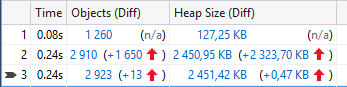
\includegraphics[scale=1]{performance-node-reuse-scenario1-1}
\caption{Memory impact comparison when parsing two identical syntax trees}
\label{img:performance-node-reuse-scenario1-1}
\end{figure}

\begin{figure}[H]
\centering
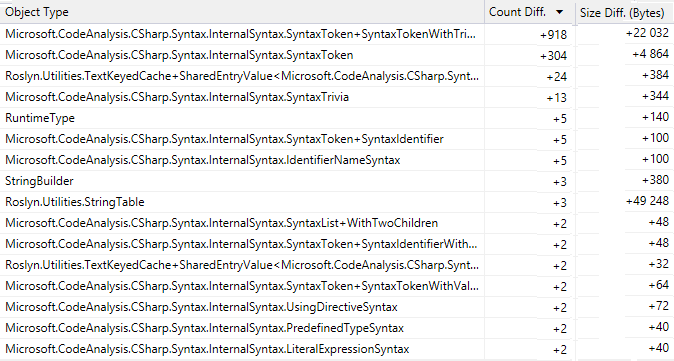
\includegraphics[scale=0.85]{performance-node-reuse-scenario1-2}
\caption{Memory impact of the first parsing session with identical trees}
\label{img:performance-node-reuse-scenario1-2}
\end{figure}

\begin{figure}[H]
\centering
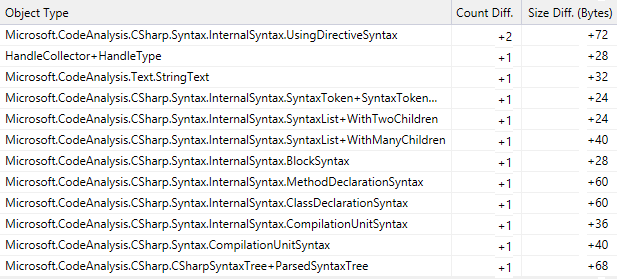
\includegraphics[scale=0.95]{performance-node-reuse-scenario1-3}
\caption{Memory impact of the second parsing session with identical trees}
\label{img:performance-node-reuse-scenario1-3}
\end{figure}

\textbf{Conclusion:} The first parsing session creates a lot of different objects while the next session only creates a relative tiny amount of new objects. An interesting aspect to note here is the kind of objects we see created in that first run (see figure \ref{img:performance-node-reuse-scenario1-2}): every token is cached when that first parsing session starts which causes a lot of initial allocations. 
When we look further down the list of allocated objects we also see caches, the parser, specific object pools, factories and a lot more. However when we now look at the second parsing session and see how it affects the heap we see none of this: there are a few new nodes representing the broad lines of the tree but no new tokens, identifiers, parsers, caches, etc have been allocated.


\item \textbf{Scenario 2:} Parsing two slightly different syntax trees

\textbf{Expectation:} Corresponding to the previous experiment, we expect a lot of allocations in the first parsing session. The second parsing session should display a slightly higher amount of newly allocated objects than in the first experiment but it should still be relatively little considering most of the allocations came from tree-independent work like populating caches and creating parsers.

\textbf{Demonstration:} 

\lstset{style=csharp, caption={Parsing two slightly different syntax trees}}
\begin{lstlisting}
internal class Experiment2
{
	public const string tree1 = @"
using System;
using System.Text;

class MyClass 
{
    void MyMethod()
    {
        int result = 2 + 2;
        Console.WriteLine(result);
    }
}";

	public const string tree2 = @"
using System;
using System.Text;

class MyClass 
{
    private string myString = ""hello"";

    void MyMethod()
    {
        int result = 2 + 2;
        Console.WriteLine(result);
    }
}";

	private static void Main(string[] args)
	{
		var obj1 = CSharpSyntaxTree.ParseText(tree1);
		var obj2 = CSharpSyntaxTree.ParseText(tree2);
	}
}
\end{lstlisting}

\textbf{Results:}

\begin{figure}[H]
\centering
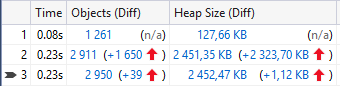
\includegraphics[scale=1]{performance-node-reuse-scenario2-1}
\caption{Memory impact comparison when parsing two slightly different syntax trees}
\label{img:performance-node-reuse-scenario2-1}
\end{figure}

\begin{figure}[H]
\centering
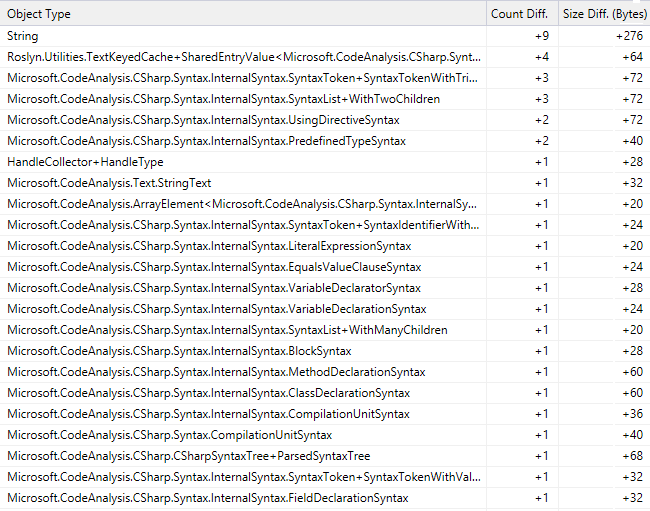
\includegraphics[scale=0.80]{performance-node-reuse-scenario2-2}
\caption{Memory impact of the second parsing session with slightly different syntax trees}
\label{img:performance-node-reuse-scenario2-2}
\end{figure}

\textbf{Conclusion:} As expected there are indeed more additional allocations in experiment 2 compared to experiment 1 (39 vs 13 respectively) which is still dwarfed by the initial allocation of 1650 objects. What we can see in figure \ref{img:performance-node-reuse-scenario2-2} are the additional string allocations and the syntax tree that makes up a field declaration (\texttt{FieldDeclarationSyntax}, \texttt{VariableDeclarationSyntax}, \texttt{VariableDeclaratorSyntax}, and so on).

\item \textbf{Scenario 3:} Iterating through the nodes of a tree

\textbf{Expectation:} We know that red nodes are materialized lazily: they have a trivial structure when the green node is constructed and get expanded to full-fledged red nodes only when this is requested. By retrieving all the descendent nodes from the root of the tree, we expect a lot of extra allocations (relative to previous experiments). If we look at previous results we can tell they are all green nodes because the objects are contained in the \texttt{InternalSyntax} namespace. By materializing, we should find allocations from objects based in the \texttt{Syntax} namespace -- the red nodes that are exposed through APIs.

\textbf{Demonstration:} 

\lstset{style=csharp, caption={Iterating through the nodes of a tree}}
\begin{lstlisting}
internal class Experiment3
{
    public const string tree1 = @"
using System;
using System.Text;

class MyClass 
{
    void MyMethod()
    {
        int result = 2 + 2;
        Console.WriteLine(result);
    }
}";
    private static void Main(string[] args)
	{
		var obj1 = CSharpSyntaxTree.ParseText(tree1);
		var objects = obj1.GetRoot()
										  .DescendantNodesAndSelf()
											.ToArray();
	}
}
\end{lstlisting}

\textbf{Results:}

\begin{figure}[H]
\centering
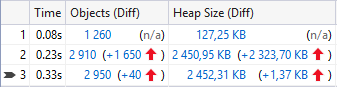
\includegraphics[scale=1]{performance-node-reuse-scenario3-1}
\caption{Memory impact comparison when materializing red nodes}
\label{img:performance-node-reuse-scenario3-1}
\end{figure}

\begin{figure}[H]
\centering
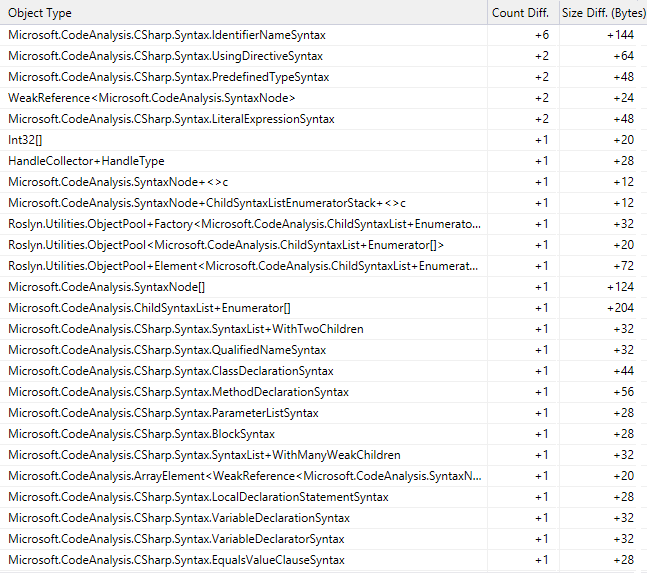
\includegraphics[scale=0.80]{performance-node-reuse-scenario3-2}
\caption{Memory impact when materializing red nodes}
\label{img:performance-node-reuse-scenario3-2}
\end{figure}

\textbf{Conclusion:} We can see that a significant amount of allocations has occurred by iterating through our syntax tree. These objects are almost all located in the \texttt{Syntax} namespace which confirms our expectation that we're dealing with red nodes. It's interesting to notice that every type that existed in our green tree now created the corresponding type in the red tree. We also see the \texttt{WeakReference} in play which we will discuss in section \ref{sec:weak-references}.




\end{itemize}
\subsection{Weak references}
\label{sec:weak-references}

\epigraph{A weak reference, simply put, is a reference that isn't strong enough to force an object to remain in memory. Weak references allow you to leverage the \gls{gc}'s ability to determine reachability for you, so you don't have to do it yourself.}
{\textit{Ethan Nicholas \\ \footnotesize{Understanding Weak References\protect\footnotemark}}}

\footnotetext{http://weblogs.java.net/blog/enicholas/archive/2006/05/understanding\_w.html}

As we talked about before in section \ref{sec:small-nodes}, C\# is a \gls{managedlanguage} that manages its memory usage with the \glslink{gc}{GC}. In essence it boils down to this: if an object has no references it is eligible for Garbage Collection and the \glslink{gc}{GC} will mark it as such so it can be cleaned up in the next iteration. You might have guessed by the title of the section that the above explanation should actually specify it as \textit{strong references} rather than just \textit{references}. A "strong reference" is the default reference type we typically use when referencing another object.

A \texttt{WeakReference} is a construct that allows us to reference an object but if the \glslink{gc}{GC} decides to clean up that reference it can do so without a problem. You notice from this description that it is perfectly suited for a caching mechanism: that's basically the same result as when we create a cache with a certain size -- the size is supposed to prevent us from reaching memory issues.

In section \ref{sec:rg-trees-solution} we already talked shortly about \gls{syntax} highlighting in the \gls{ide}: scrolling through the editor will cause the \gls{syntaxtree} to become materialized which means creating new objects to represent those syntactic constructs. However once a part of the tree leaves the window of the user there is no point in keeping it materialized anymore since the user can't see it anyway. At this point you want those unnecessary materialized nodes to be garbage collected but there is one major problem: nodes are referenced by their parent and its children. If we would use traditional strong references we would never be able to collect any of these objects.

One major area in which this technique is used is when it comes to a method body. Method bodies are in essence a group of statements. While it can be very useful to have information such as the method's definition available while programming, the exact contents of that method its implementation are less important -- this makes it a perfect target to use weak references.

This is implemented in the \texttt{SyntaxList.WithManyWeakChildren} type. It works very straightforward: by storing an array with as type a \texttt{WeakReference<SyntaxNode>} we are already done: now these syntax nodes will be able to be \glslink{gc}{GC}'d if the \glslink{gc}{GC} marks them and no strong references exist to those particular nodes.

\lstset{style=csharp, caption={SyntaxList.WithManyWeakChildren.\_children}}
\begin{lstlisting}
private readonly 
	ArrayElement<WeakReference<SyntaxNode>>[] _children;
\end{lstlisting}

\noindent In the base type \texttt{SyntaxList.WithManyChildrenBase} we can see how the creation of the red node is delegated:

\lstset{style=csharp, caption={SyntaxList.WithManyWeakChildrenBase.CreateRed}}
\begin{lstlisting}
internal override SyntaxNode CreateRed(SyntaxNode parent, 
																			 int position)
{
	var p = parent;
	if (p != null && p is CSharp.Syntax.BlockSyntax)
	{
		var gp = p.Parent;
		if (gp != null && 
				(gp is CSharp.Syntax.MemberDeclarationSyntax || 
				 gp is CSharp.Syntax.AccessorDeclarationSyntax))
		{
			return new 
				SyntaxList.WithManyWeakChildren(this, 
																				parent, 
																				position);
		}
	}

	if (this.SlotCount > 1 && HasNodeTokenPattern())
	{
		return new 
			SyntaxList.SeparatedWithManyChildren(this, 
																					 parent, 
																					 position);
	}
	else
	{
		return new 
			SyntaxList.WithManyChildren(this, 
																	parent, 
																	position);
	}
}
\end{lstlisting}

\subsection{Object pooling}
\label{sec:object-pooling}

In chapter \ref{sec:object-reuse} we've discussed a specific approach at minimizing the amount of objects created. In this section we will take a look at a more general implementation of this idea. While nodes and tokens are at the very core of the Roslyn code base, they're not the only objects we'll create. 

When creating a lexer, one of the major tasks you're performing is reading source code and creating strings. If you would intermittently concatenate strings, this would increase memory pressure by a lot: every concatenation using \verb|+| creates a new string but you might only be interested in the result\footnote{https://msdn.microsoft.com/en-us/library/2839d5h5(v=vs.110).aspx}. 
However creating a new \verb|StringBuilder| object every time you want to concatenate strings is an expensive operation as well: since a lot of string concatenation is done, a lot of distinct \verb|StringBuilder| instances will be created and you again have the issue as described before. The solution here is to take pooling one step further: every type can be pooled through the \verb|ObjectPool<T>| class.\parencite{Warren2014} This provides a generic implementation of the object pooling pattern and will be used through intermediate classes.

An accurate description of this class' workings can be found in its documentation\footnote{\url{https://github.com/dotnet/roslyn/blob/b908b05b41d3adc3b5e81f8cf2d0055c13e4a1f6/src/Compilers/Core/SharedCollections/ObjectPool\%601.cs}}:

\begin{quotation}
Generic implementation of object pooling pattern with predefined pool size limit. The main
purpose is that limited number of frequently used objects can be kept in the pool for
further recycling.

Notes: 

1) it is not the goal to keep all returned objects. Pool is not meant for storage. If there
   is no space in the pool, extra returned objects will be dropped.

2) it is implied that if object was obtained from a pool, the caller will return it back in
   a relatively short time. Keeping checked out objects for long durations is ok, but 
   reduces usefulness of pooling. Just new up your own.

Not returning objects to the pool in not detrimental to the pool's work, but is a bad practice. 
Rationale: 
   If there is no intent for reusing the object, do not use pool - just use "new". 
\end{quotation}

An interesting addition here is the implementation of \verb|SharedPools|. As the name indicates, this is a class that manages the sharing of object pools. There are two ways to use this class:

\begin{itemize}
\item As a single, standalone pool

This does not share the pool but instead just makes it easier to create your object pools. For this purpose you can choose between a small pool (20 elements) and a big pool (100 elements). For example in the case of a small pool you call

\lstset{style=csharp, caption={SharedPools.Default<T>}}
\begin{lstlisting}
public static ObjectPool<T> Default<T>() 
																where T : class, 
																					new()
{
	return DefaultNormalPool<T>.Instance;
}
\end{lstlisting}

This method, in turn, will lazily create a new pool the first time a pool of that type is requested. This pool will defer to the beforementioned \verb|ObjectPool| implementation:

\lstset{style=csharp, caption={SharedPools.DefaultNormalPool<T>}}
\begin{lstlisting}
private static class DefaultNormalPool<T> 
																where T : class, 
																					new()
{
	public static readonly ObjectPool<T> Instance = 
		new ObjectPool<T>(() => new T(), 20);
}
\end{lstlisting}

\item As a shared pool

Taking the entire idea another step further, you can also share the pools themselves. This is useful to share data inside the pools: if in one parsing session you create a string "using" then it would be nice to re-use that in another parsing session. This follows the same idea of the statically shared \verb|TextKeyedCache| pool as we talked about in section \ref{sec:re-use-tokens} but expands this usage across all types due to its generic nature. Here again we see two separate usages:

\subitem As a pre-defined pool

Inside the \verb|SharedPools| we have a few pre-defined pools for general use cases. One of those is \verb|StringIgnoreCaseHashSet| which provides a hashset pool that compares its elements case-insensitively.

\lstset{style=csharp, caption={SharedPools.StringIgnoreCaseHashSet}}
\begin{lstlisting}
public static readonly 
	ObjectPool<HashSet<string>> StringIgnoreCaseHashSet =
	new ObjectPool<HashSet<string>>(
		() => new HashSet<string>(
							StringComparer.OrdinalIgnoreCase), 20);
\end{lstlisting}

\subitem As a pre-defined type

There are also specific types that provide some type-specific behaviour. An example of this is the \verb|StringBuilderPool|:

\lstset{style=csharp, caption={StringBuilderPool}}
\begin{lstlisting}
internal static class StringBuilderPool
{
	public static StringBuilder Allocate()
	{
		return SharedPools.Default<StringBuilder>()
										  .AllocateAndClear();
	}
	
	public static void Free(StringBuilder builder)
	{
		SharedPools.Default<StringBuilder>()
							 .ClearAndFree(builder);
	}
	
	public static string ReturnAndFree(
													StringBuilder builder)
	{
		SharedPools.Default<StringBuilder>()
							 .ForgetTrackedObject(builder);
		return builder.ToString();
	}
}
\end{lstlisting}

\end{itemize}
\newpage
\subsection{Specialized collections}
\label{sec:specialized-collections}

Collections in the .NET framework are heavily optimized by themselves already but it is done so in a general manner: in the end, the .NET framework will be used by many different people so optimizations have to be weighed against a lot of different scenarios. By creating your own specialized collections, you have the possibility to cut corners that might not be applicable in your domain's scenario. In its crudest form: if you have a \texttt{null} check inside the collection's operations but you know for sure that that can never be \texttt{null} then that is an instruction you can skip. Another important reason to use your own custom collections is to formalize the specific behaviour of your domain that belongs to a collection. 

\subsubsection{IdentifierCollection}
\label{sec:spec-coll-identifiercollection}

An example of the latter can be found in the form the \texttt{IdentifierCollection}. This class acts as a wrapper around a \texttt{Dictionary} that maps a certain key to one or more alternative spellings of that key. While in essence nothing more than a mapper between key and value, it provides more intuitive methods to interact with such as \texttt{AddIdentifier}, \texttt{AddInitialSpelling} and \texttt{AddAdditionalSpelling}.
In this case, we can see a performance consideration in the way it stores the alternative identifiers: the backing \texttt{Dictionary} is actually mapping a \texttt{string} to an \texttt{object} instead of an array as one would expect. The reason this is done is to avoid having to allocate an array when there is just one alternative identifier -- now we can just define it as a \texttt{string} without the need for an array.

\clearpage

\begin{minipage}{\linewidth}
We can see this consideration reflected when we try to add a new spelling to a given key:

\lstset{style=csharp, caption={IdentifierCollection.AddAdditionalSpelling}}
\begin{lstlisting}
private void AddAdditionalSpelling(string identifier, 
																	 object value)
{
	// Had a mapping for it.  It will either map to a single 
	// spelling, or to a set of spellings.
	var strValue = value as string;
	if (strValue != null)
	{
		if (!string.Equals(identifier, 
											 strValue, 
											 StringComparison.Ordinal))
		{
			// We now have two spellings. Create a collection 
			// for that and map the name to it.
			_map[identifier] = new HashSet<string> 
				{ identifier, strValue };
		}
	}
	else
	{
		// We have multiple spellings already.
		var spellings = (HashSet<string>)value;

		// Note: the set will prevent duplicates.
		spellings.Add(identifier);
	}
}
\end{lstlisting}
\end{minipage}

Notice also the note on line 20: smart usage of existing collections reduces the complexity of our own code.

\newpage
\subsubsection{CachingDictionary}
\label{sec:spec-coll-cachingdictionary}

Another implementation is the \texttt{CachingDictionary}. As its name indicates, it represents an in-memory caching mechanism based on the \texttt{Dictionary} collection. There is a very interesting implementation detail here: the backing dictionary is a \texttt{ConcurrentDictionary} meaning its exposed methods are \gls{threadsafe}. However, when the backing dictionary is full, it actually swaps that out for a normal \texttt{Dictionary} to allow for less-expensive read-operations without the thread-safety overhead.

\lstset{style=csharp, caption={CachingDictionary.IsNotFullyPopulatedMap}}
\begin{lstlisting}
private static bool IsNotFullyPopulatedMap
		(IDictionary<TKey,	ImmutableArray<TElement>> map)
{
	return 
		map == null || 
		map is 
		 ConcurrentDictionary<TKey, ImmutableArray<TElement>>;
}
\end{lstlisting}
\newpage
\subsection{LINQ}
\label{sec:linq}

\epigraph{The code regions which take the most execution time are called \textit{hot spots}. The hot spots are the best places to tune and optimize because a little bit of effort on making a hot spot faster can have a big pay-off. It’s not worth spending engineering effort on a bit of code that executes only once or doesn’t take much time.}
{\textit{Paul J. Drongowski \\ \footnotesize{PERF tutorial: Finding execution hot spots\protect\footnotemark}}}

\footnotetext{http://sandsoftwaresound.net/perf/perf-tutorial-hot-spots/}

An explicit performance consideration mentioned in the "Contributing Code" guidelines on the project's Github page\footnote{\url{https://roslyn.codeplex.com/wikipage?title=How\%20to\%20Contribute}} explicitly mentions \gls{linq}\footnote{LINQ: Language-Integrated Query, syntax features to query data}:

\begin{quote}
Avoid allocations in \gls{compiler} hot paths:
\begin{itemize}
\item Avoid \gls{linq}.
\item Avoid using \texttt{foreach} over collections that do not have a \texttt{struct} enumerator.
\item Consider using an object pool. There are many usages of object pools in the \gls{compiler} to see an example.
\end{itemize}
\end{quote}

It's already clear that the main idea here is minimizing allocations made -- an overarching theme which we have also discussed in previous sections. In this section we will focus on \gls{linq} and some of the performance implications that come with it. The two other bullet points also have to do with memory allocation: both concern memory allocation on the heap which will eventually trigger a \gls{gc}.

The concern here is that \gls{linq} adds an unacceptable overhead in the team's eyes. This overhead is inherent to \gls{linq}: you make a trade-off between memory and performance impact and instead end up with much more readable code. 

As means of a simple test, we'll take a look at a snippet of code and its \gls{linq} alternative and compare their memory impact. We'll create two memory snapshots and see how many extra objects have been created for each implementation. It should obviously be noted that not all \gls{linq} statements are equally wasteful and in some scenarios \gls{linq} can even make sure there is less memory impact.

The code we use to test can be found in listing \ref{lst:linq-memory} and adds 3 items from one list to another based on a certain condition. One approach uses a \gls{linq} query while the other uses a \texttt{foreach} loop which is basically the unrolled equivalent of the former. The heap snapshots in figures \ref{img:performance-linq-memlinq} and \ref{img:performance-linq-memloop} give use a clear view of what objects are being allocated along the way: we can see that constructing the \gls{linq} query creates two new objects of types \texttt{Enumerable+WhereListIterator<Int32>} and \texttt{Func<Int32, Boolean>}, representing the \texttt{Where} structure and the where condition respectively. Additionally there is an object \texttt{HandleCollector+HandleType} which is overhead created by the \glslink{gc}{GC}. 

When we take a look at the next snapshot we can see that after Garbage Collecting and running our \texttt{foreach} loop, we now notice that we only create the overhead object and that the \texttt{WhereListIterator} has been Garbage Collected. You might wonder what happened to the \texttt{Func} -- in the end, that condition isn't referenced anywhere anymore and as such it should be eligible for collection. The optimization at play here is that the \gls{compiler} caches lambdas if they adhere to certain characteristics such as not using a local variable\footnote{http://stackoverflow.com/a/6280711/1864167}. By using this lambda in our code we now have an object that will live for a long time and, by definition, increase memory pressure. Using the caching technique keeps this memory pressure limited but knowing that there are at least one or two object allocations for the simplest of \gls{linq} queries makes it easy to see why they should be avoided in hot paths.


\begin{figure}
\centering
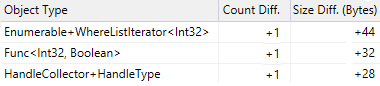
\includegraphics[scale=1]{performance-linq-memlinq}
\caption{Memory impact when comparing the LINQ query to the baseline}
\label{img:performance-linq-memlinq}
\end{figure}

\begin{figure}[h]
\centering
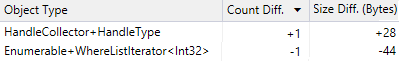
\includegraphics[scale=1]{performance-linq-memloop}
\caption{Memory impact when comparing the loop to the LINQ query}
\label{img:performance-linq-memloop}
\end{figure}

\lstset{style=csharp, caption={Comparing LINQ memory impact}}
\begin{lstlisting}[label={lst:linq-memory}]
static void Main(string[] args)
{
    // Setting baseline snapshot
    var list1 = new List<int> {4862, 6541, 7841};
    var list2 = new List<int>(list1.Count);
    var list3 = new List<int>(list1.Count);

    // First snapshot: LINQ usage
    list2.AddRange(list1.Where(item => item > 5000 && 
																			 item < 7000));

    // Second snapshot: foreach-loop
    foreach (var item in list1)
    {
        if (item > 5000 && item < 7000)
        {
            list3.Add(item);
        }
    }
}
\end{lstlisting}



